% fig2-cache-trajectory.tex — §7 cache calibration visualisation (RC-07)
% Data source: data/aggregated/cache-stats.csv (summary metrics)
% Since we have a summary (not daily time-series), we render a bar comparison
% of cache creation vs cache read tokens (log scale to make the ratio visible).
% Style: print-safe, width=0.85\textwidth, height=6cm

\begin{figure}[ht]
\centering

% Summary stats from cache-stats.csv:
%   cache_creation_total_tokens = 5807869
%   cache_read_total_tokens     = 60370940
%   read_to_creation_ratio      = 10.39
%   savings_vs_no_caching       = 0.786

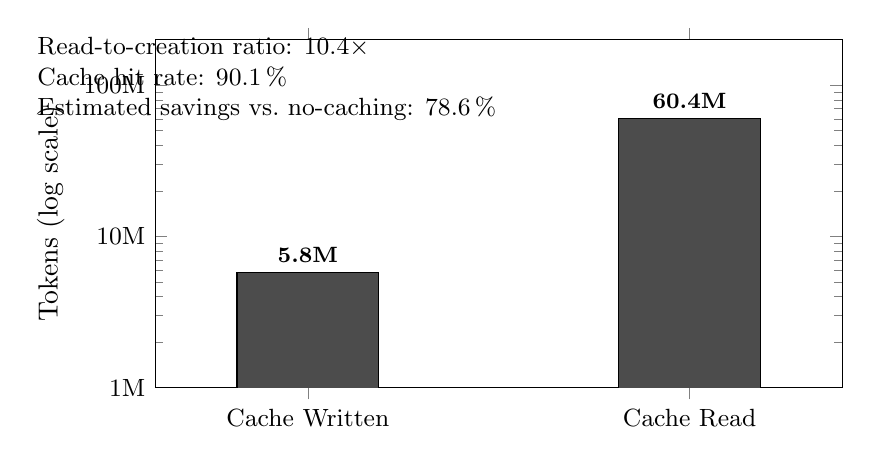
\begin{tikzpicture}
\begin{axis}[
  ybar,
  width=0.85\textwidth,
  height=6cm,
  bar width=1.8cm,
  ymode=log,
  log ticks with fixed point,
  ylabel={Tokens (log scale)},
  xtick=data,
  symbolic x coords={Cache Written, Cache Read},
  xticklabel style={font=\small},
  ymin=1000000,
  ymax=200000000,
  ytick={1000000,10000000,100000000},
  yticklabels={1M,10M,100M},
  yticklabel style={font=\small},
  nodes near coords,
  nodes near coords style={
    font=\footnotesize\bfseries,
    /pgf/number format/fixed,
    /pgf/number format/precision=1,
  },
  point meta=explicit symbolic,
  enlarge x limits=0.4,
  legend style={
    at={(0.97,0.97)},
    anchor=north east,
    font=\small,
    draw=black,
  },
]
\addplot+[
  fill=black!70,
  draw=black,
  every node near coord/.append style={color=black},
] coordinates {
  (Cache Written, 5807869)   [5.8M]
  (Cache Read,   60370940)   [60.4M]
};
\end{axis}
% Annotate ratio
\node[anchor=north west, font=\small] at (current bounding box.north west)
  {%
    \begin{minipage}{0.5\textwidth}
      \raggedright
      Read-to-creation ratio: $10.4\times$\\
      Cache hit rate: 90.1\,\%\\
      Estimated savings vs.\ no-caching: 78.6\,\%
    \end{minipage}
  };
\end{tikzpicture}

\caption{%
  Prefix-cache token volumes over the 7-day window
  (\texttt{cache\_creation\_input\_tokens} vs.\ \texttt{cache\_read\_input\_tokens},
  log scale).
  The $10.4\times$ read-to-creation ratio and 90.1\,\% hit rate confirm sustained
  cache reuse within the 5-minute TTL window, yielding a 78.6\,\% cost reduction
  vs.\ no-caching baseline.
  Source: \texttt{data/aggregated/cache-stats.csv}.%
}
\label{fig:cache-trajectory}
\end{figure}
